\documentclass[11pt]{article}
\usepackage{c://pctex/activity}

\lhead{}
\chead{\textbf{\large{Exercise 17 -- Section 7.2\\Examples of Relations with Certain Properties}}}
\rhead{}
\lfoot{\emph{Mathematical Reasoning: Writing and Proof, Third Ed.} \\Ted Sundstrom}
\cfoot{}
\rfoot{\copyright \the\year\, by Pearson Education, Inc.\\}
%\renewcommand{\labelenumi}{\textbf{\arabic{enumi}.}}

\begin{document}
\begin{enumerate}
  \item A relation $R$ on a set $A$ is not a circular relation provided that there exist $x$, $y$, and $z$ in $A$ such that $x \mathrel{R} y$, $y \mathrel{R} z$, and $z \not\mathrel{R} x$.  
  \item \qquad

\begin{center}
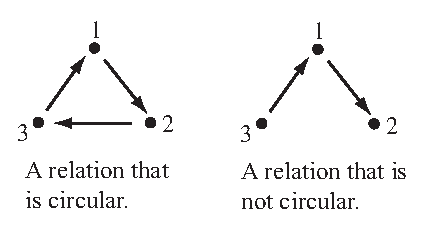
\includegraphics{fig-sec72-1.eps}
\end{center}
  
\item \qquad

\begin{center}
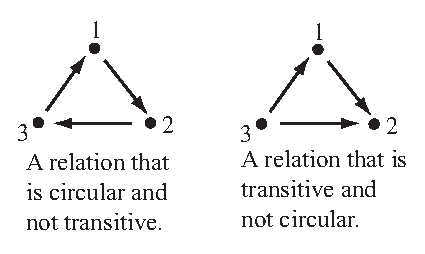
\includegraphics{fig-sec72-2.eps}
\end{center}

\item \textbf{Proposition}.  A relation $R$ on a set $A$ is an equivalence relation if and only if it is reflexive and circular.

\begin{myproof}
We assume that $R$ is a relation on a set $A$ and will prove that $R$ is an equivalence relation if and only if it is reflexive and circular.  

We first assume that $R$ is an equivalence relation.  So $R$ is reflexive and we must prove that $R$ is circular.  So let $x, y, z \in A$ and assume that $x \mathrel{R} y$ and $y \mathrel{R} z$.  Since $R$ is transitive, we conclude that $x \mathrel{R} z$ and hence, since $R$ is also symmetric, $z \mathrel{R} x$.  Hence, $R$ is circular and this proves that if $R$ is an equivalence relation, then $R$ is reflexive and circular.

We now assume that $R$ is reflexive and circular.  To prove that $R$ is an equivalence relation, we must prove that $R$ is symmetric and transitive.  We will first prove that $R$ is symmetric and so we let $u,v \in A$ and assume that $u \mathrel{R} v$.  Since $R$ is symmetric, $u \mathrel{R} u$ and so we now have $u \mathrel{R} u$ and $u \mathrel{R} v$.  Since $R$ is circular, we can now conclude that $v \mathrel{R} u$ and hence, $R$ is symmetric.  To prove that $R$ is transitive, we let $u, v, w \in A$ and assume that $u \mathrel{R} v$ and 
$v \mathrel{R} w$.  Since $R$ is circular, we can conclude that $w \mathrel u$ and since $R$ is reflexive, we conclude that $u \mathrel{R} w$.  Therefore, $R$ is transitive and this proves that if $R$ is reflexive and symmetric, then $R$ is an equivalence relation.
\end{myproof}



\item A relation $R$ on a set $A$ is not antisymmetric provided that there exist $x, y \in A$ such that $x \mathrel{R} y$, $y \mathrel{R} x$, and $x \ne y$.

\newpage
\item \qquad

\begin{center}
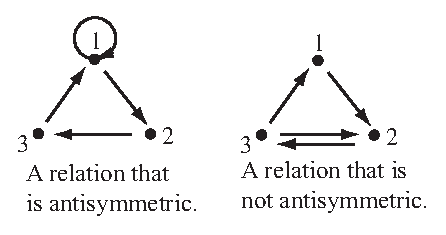
\includegraphics{fig-sec72-3.eps}
\end{center}



\item \textbf{Proposition}.  If a relation $R$ on a set $A$ is both symmetric and transitive, then $R$ is transitive.

\textbf{Outline of a Proof}.  Assume that $R$ is both symmetric and antisymmetric.  We will prove that $R$ is transitive.  So let $a, b, c \in A$ and assume that $a \mathrel{R} b$ and 
$b \mathrel{R} c$. Since $R$ is symmetric, we can conclude that $b \mathrel{R} a$.  So we have 
$a \mathrel{R} b$ and $b \mathrel{R} a$.  Since $R$ is antisymmetric, this implies that 
$a = b$.  However, we then have $a = b$ and $b \mathrel{R} c$.  Hence, $a \mathrel{R} c$ and we have proven that $R$ is transitive.

\textbf{Proposition}.  If a relation $R$ on a set $A$ is both symmetric and antisymmetric, then $R$ is reflexive.

This is false.  A counterexample is $A = \{ x, y \}$ and $R = \{ (x, x) \}$.  This relation is both symmetric and antisymmetric but is not reflexive.

\end{enumerate}



\end{document}
